\documentclass{article}

\usepackage{ijcai13}
\usepackage{times}
\usepackage{latexsym}
\usepackage{float} 
\usepackage{graphicx}

\begin{document}

\title{Modélisation d'évacuation d'une salle de cinéma}
\author{
Romain Kugler \& Yann Martin D'Escrienne\\
Université Nice-Sophia Antipolis\\
2019}

\maketitle

\begin{abstract}
Cet article porte sur l’évacuation d’urgence d’une salle de cinéma. Dans celui-ci notre étude utilise une simulation {\it Netlogo} et consiste à faire varier certains paramètres importants d’une évacuation, tels que le nombre de sortie, la densité d’individus dans la salle, la zone du départ de l’incendie et la présence d’obstacle devant les sorties principales. Tout cela dans le but de trouver d'obtenir une évacuation rapide et sans pertes humaines grâce à l'interprétation de nos données. 

\end{abstract}

\section{Introduction}
\subsection{Contexte}
L’évacuation d’une salle ou d’un bâtiment lors d’un sinistre peut-être catastrophique et engendrer de nombreux décès si la disposition de la salle ne s’y prête pas et que la panique envahit les individus cherchant à fuir (bousculade, piétinement). Il faut donc éviter d’arriver à ce genre de situation en optimisant l’évacuation pour la rendre la plus fluide possible. Également limiter au maximum les pertes humaines, ce qui est le réel objectif.  
Pour cela il faut notamment identifier les paramètres importants afin d’obtenir un temps minimal d’évacuation, mais surtout trouver les conditions qui influent le plus sur le nombre de décès. 
Il en ressort donc certaines questions fondamentales. 

\subsection{Questions scientifiques}
La question centrale et naturelle de cette article est donc :\\
{\bf Comment optimiser une évacuation ?}\\
Autrement dit : {\bf Comment obtenir un temps d'évacuation minimal ?}
et également {\bf À quel endroit le danger est-il le plus important ?}\\
Nous allons répondre à cette question à l’aide de différents outils tel que Netlogo, un langage de programmation et environnement de modélisation pour le développement de système multi-agents et R, un langage de programmation destiné aux statistiques.

\section{Modelisation} 
\subsection{Description du modèle} 
Pour limiter les mesures, nous avions décidés que la modélisation se situerai dans une salle de cinéma de taille moyenne et que le danger choisi serait le feu. En effet il est le plus commun et mortel des cas possibles et donc celui qui donnait le plus d’impact dans nos mesures.

\subsubsection{Paramètres}
Après nos réflexions sur les paramètres influençant le plus une évacuation nous avons choisi les suivants : la {\bf densité} d’individus installés dans la salle, le {\bf nombre} de sortie, celui-là étant le plus intuitif, et la présence ou non d’un {\bf obstacle} devant les sorties où le flux humain serait le plus important.

Concernant les conditions influant sur les pertes humaines nous avons choisi {\bf l'emplacement} de départ du feu, c'est à dire la zone où celui-ci se déclarait dans notre salle.

\subsubsection{Mesures}
Quant aux mesures elles furent plutôt intuitives. Pour l'influence des paramètres: le {\bf temps d’évacuation total}, c’est à dire le temps qu’il faut pour que tous les individus pour quitter la salle,
le {\bf nombre d’évacués} à un temps donné, et un {\bf temps moyen} de sortie de plusieurs simulations. Pour mesurer l’importance du danger, nous avons choisis de façon naïve le {\bf nombre de morts} durant l’incendie. 

\subsection{Hypothèses simplificatrices} 
Comme hypothèses simplificatrices pour notre simulation nous avons décidés de considérer les individus comme identiques, c’est à dire qu’ils possèdent tous la même vitesse de déplacement et la même taille.

Un monde en trois dimensions étant trop complexe sur {\it Netlogo} nous avons représentés la salle par un monde en deux dimensions. Cela implique que les murs, les sièges, et le feu sont représentés par des patchs ({\em cases de notre monde 2D}).

Nos individus ne peuvent pas être déplacés par autrui, c’est à dire qu’ils ne peuvent se faire pousser par les autres, même si cela aurait pu influencer sur le nombre de blessés et de morts.

Nos sorties ont été toutes identiques étant donné la petitesse de notre salle, une sortie plus grande aurait tellement accéléré le temps d’évacuation que l’influence des autres paramètres aurait été nulle.\\\\
Toutes ces hypothèses simplificatrices nous permettent donc d’obtenir une simulation fluide permettant tout de même des mesures effectives. 



\section{Simulation} 
\subsection{Cadre expérimental} 
\begin{figure}[H]
	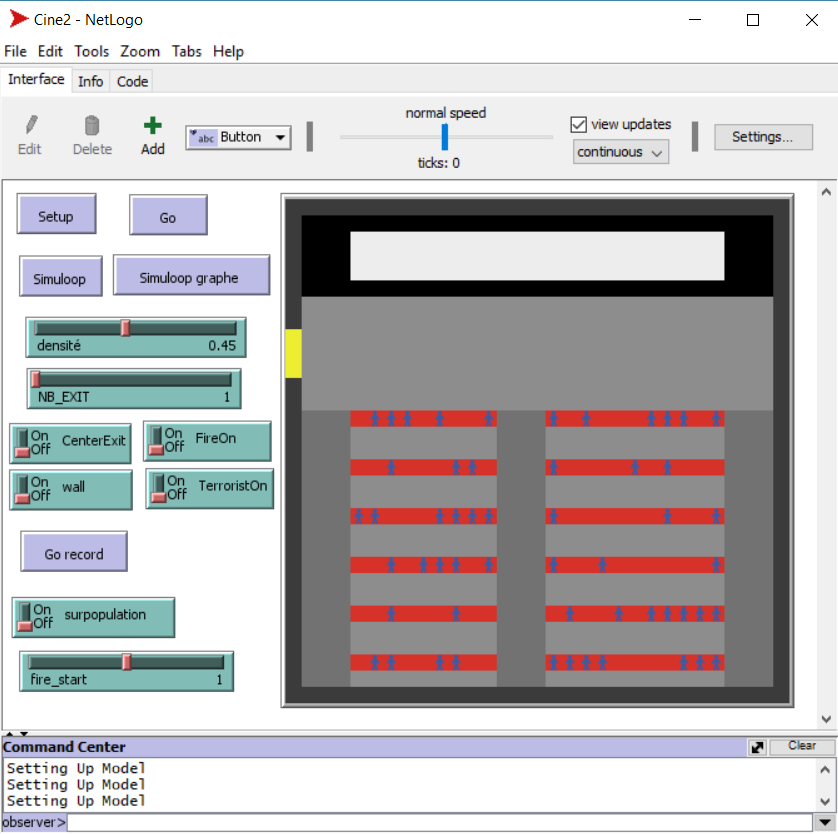
\includegraphics[scale=0.5]{capture.PNG}
  \centering
	\caption{Salle de cinéma}
 	\label{pic: capture}
\end{figure}

La {\it figure1} ci-dessus correspond à notre simulation sous {\it Netlogo}. Notre salle fait 30x30 patchs, où un patch de notre simulation correspond à 1m réel, donc 90m$^2$. Le haut de la simulation correspond au bas de la salle.

Elle est représentée par les éléments suivants : des murs ({\it en noir}), des sièges ({\it en rouge}), des escaliers ({\it en gris foncé}) ainsi qu'une ou plusieurs sorties ({\it en jaune}) selon {\it NB\_EXIT (Fig 1)}.
La partie supérieure de la salle représente la scène et l'écran et n'est pas accessible aux turtles. Les sièges et murs sont eux aussi considérés comme des obstacles sur lesquels les turtles ne peuvent se déplacer.

Les individus sont représentés par les turtles bleus. Lors de l'initialisation, la position des turtles sur les sièges est déterminée de manière aléatoire et il ne peut y avoir qu'une turtle par siège. Leur nombre dépend de la valeur {\it densité} modifié grâce au {\it slider (Fig 1)}.

Un ticks de la simulation correspond à une seconde réelle. La vitesse de déplacement des turtles est d'un patch par tick, soit un mètre par seconde. ({\em ce qui correspond à la vitesse de marche soutenue moyenne})

Les turtles agissent de manière intelligente, elles se dirigent tout d'abord vers l'escalier le plus proche puis une fois situées dans la zone devant l'écran, elle se dirigent vers la sortie la plus proche de leur position. Elle contournent les obstacles et peuvent faire demi-tour en cas de voie sans issue ({\it notamment à cause du feu}). Elles réagissent également en fonction de leur voisine, elles peuvent choisir de les contourner ou bien de ne pas bouger. De plus lorsque le feu bloque une sortie, immédiatement, les turtles l'abandonnent et se dirigent vers l'autre. 

\begin{figure}[H]
	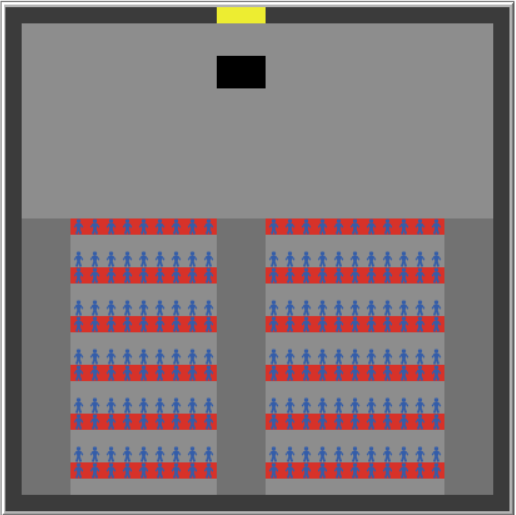
\includegraphics[scale=0.3]{center.PNG}
  \centering
	\caption{Disposition de la salle avec CenterExit et Wall}
 	\label{pic: Feu}
\end{figure}
Le switch {\it CenterExit (Fig 2)} permet de créer une disposition telle que la salle possède une unique sortie au centre ({\em l'écran est retiré}).

Le switch {\it Wall (Fig 2)} créer un obstacle 3x2 patchs juste devant cette sortie. Il n'est activable que si {\it CenterExit} est actif. 

Le switch {\it Surpopulation (Fig 2)} ajoute 100 individus aux autres déjà présents.

\begin{figure}[H]
	
\includegraphics[scale=0.5]{feu_im.PNG}
  \centering
	\caption{Le feu dans la simulation}
 	\label{pic: Center}
\end{figure}

Concernant le feu ({\it Fig 3}), celui-ci est représenté en {\it orange}. Il est activé ou non selon le switch {\it FireOn (Fig 1)}. Quant à son emplacement de départ, il est aléatoire mais peut être centrer sur une zone, cela dépend de la valeur du slider {\it fire\_start (Fig 1)} : 0 pour toute la salle, 1 pour un départ dans la zone devant l'écran, 2 pour un départ entre les sièges. Il ne peux apparaitre sur un escalier, un mur, l'écran ou les sièges.
Chaque case de feu a une chance de se propager sur une des cases adjacentes selon une probabilité fixe ({\it 1 chance sur 15}). Dès qu'une turtle entre en contact avec le feu elle est immédiatement tuée.\\\\
Cette simulation nous permet donc de procéder au protocole  expérimental suivant..

\subsection{Protocole expérimental} 

Afin de répondre aux questions scientifiques posées précédemment, il fallait effectuer une série de simulations au cours desquelles nous avons fait varier les paramètres cités plus haut.

\begin{itemize}
\item Premièrement, pour mettre en évidence la relation entre densité et temps d'évacuation, nous avons réalisé plusieurs simulations en faisant varier de manière croissante la densité (de 0 à 1 par pas de 0.02) puis nous avons mesurer le temps d'évacuation de chacun des cas. 

\item Dans un second temps, nous avons fait varier le nombre de sorties et comparé les temps d'évacuation moyens obtenus.

\item Puis nous avons ajouté le feu à notre simulation pour mesurer la répartition du nombre de morts selon l'emplacement du départ du feu.

\item Enfin, avec la disposition suivante ({\it Figure 2}), nous avons mesuré le temps d'évacuation moyen sur 20 simulations, avec la présence ou non d'un obstacle devant la sortie.
Dans ce dernier cas, nous avons choisi de ne mettre qu'une sortie, et de remplir au maximum la salle pour obtenir le meilleur effet de congestion possible.
\end{itemize}

Pour réaliser nos mesures, nous avons créé des boutons ({\it Go-record, simuloop, simuloop-graphe}) appelant plusieurs fois des fonctions exportant les données obtenues dans des fichiers ".csv". 
La nature des données exportées dépendaient de l'expérience à effectuer. 

Nous avons donc réalisé différentes fonctions par expérience afin d'obtenir les données les plus concises possibles: ({\it Fig 1}) {\it go-record} enregistre le nombre de mort et d'évacué au ticks T; {\it simuloop} enregistre le nombre ticks nécessaire à l'évacuation totale; {\it simuloop-graphe} marche comme {\it simuloop} mais incrémente la densité.

Ces fichiers csv ont ensuite été traités avec des scripts écrits en R pour en extraire des statistiques et des graphiques qui vont mettre en évidence les résultats obtenus..

\section{Résultats} 
\subsection{Relation densité - Temps d'évacuation}
Même si la relation entre la densité et le temps d'évacuation semble immédiate ou intuitive, il convient toutefois d'en mesurer l'importance.

Nous avons donc incrémenter la densité comme cité plus haut et avons obtenu le graphique suivant : 
\begin{figure}[H]
	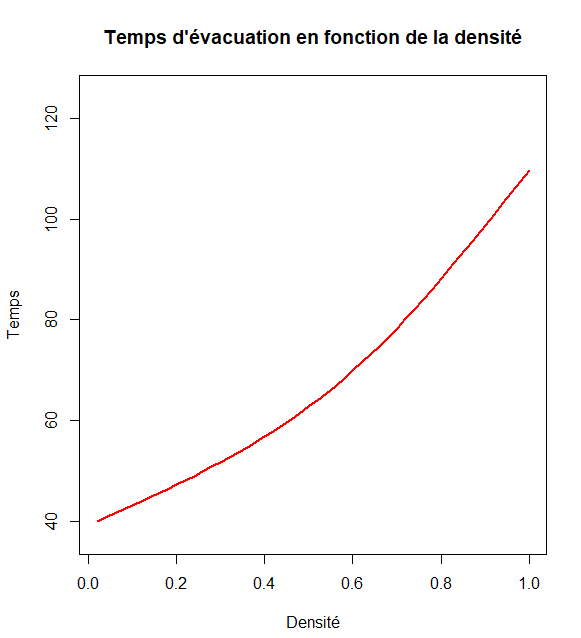
\includegraphics[scale=0.35]{densite_temps.PNG}
  \centering
	\caption{Relation entre densité et temps d'évacuation}
 	\label{pic: Densite}
\end{figure}
On remarque donc une relation quasi-linéaire entre densité et temps d'évacuation.

\subsection{Relation nombre de sorties - temps d'évacuation}
De même, le comportement du nombre d'évacués au temps T pour une et deux sorties est prévisible, néanmoins nous avons effectué les mesures pour en voir le réel impact. 

Voici le graphique obtenu :
\begin{figure}[H]
	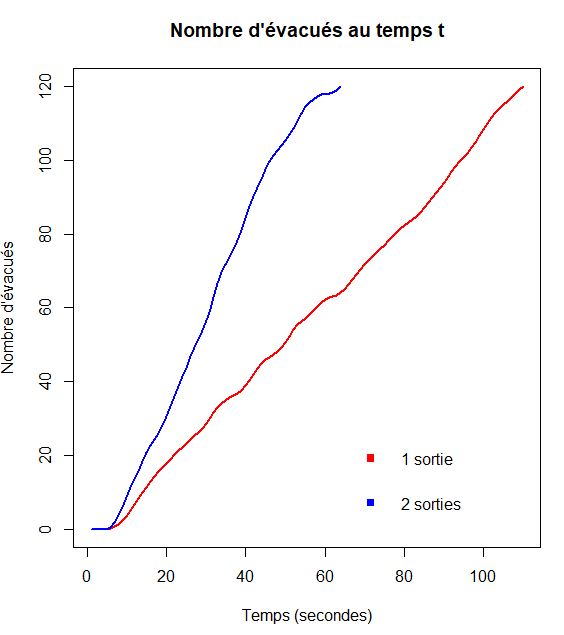
\includegraphics[scale=0.35]{nb_sortie.PNG}
  \centering
	\caption{Temps d'évacutaion en fonction du nombre de sorties}
 	\label{pic: nb_sortie}
\end{figure}

On remarque que le temps d'évacuation totale pour une sortie est environ 110 secondes ({\it courbe rouge}). Quant à la courbe pour deux sorties on obtient une évacuation totale en environ 60 secondes ({\it courbe bleue}).
On constate que le temps d'évacuation est quasiment réduit de moitié en ajoutant une deuxième sortie .

\subsection{Relation lieu de départ du feu - pertes humaines}
Nous avons effectué une série de simulations pour chacun des cas où le feu apparaissait de manière aléatoire dans deux zones concernées : devant l'écran en bas et au niveau des sièges en haut.

Une fois les simulations effectuées, les données ont été exportées puis traitées. On obtient alors le diagramme suivant:

\begin{figure}[H]
	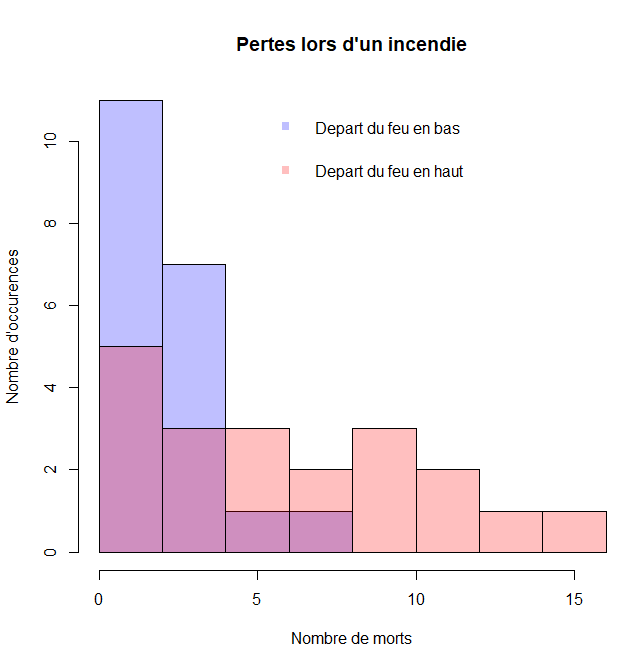
\includegraphics[scale=0.35]{graphe_nb_mort.PNG}
  \centering
	\caption{Répartition du nombre de morts}
 	\label{pic: nb_morts}
\end{figure}

On remarque ici que le nombre de pertes est beaucoup plus étalé lorsque le feu démarre devant l'écran, près de sorties ({\it en orange}), et va jusqu'à des valeurs extrêmes ({\it 16 morts}).
A contrario, lorsque le feu démarre dans la partie supérieure du cinéma ({\it en bleu}), on remarque que le nombre de morts est majoritairement compris entre 0 et 4.

\subsection{Relation Obstacle - Temps d'évacuation}
Ici nous avons donc activé l'option {\it Surpopulation} afin d'accentuer les effets de congestion au niveau de l'unique sortie placée au centre, de sorte à ce que les individus y arrivent en même temps.

Sur une moyenne de 20 simulations nous avons testé un cas avec obstacle ({\it Fig 7}) et sans obstacle ({\it Fig 8})
\begin{figure}[H]
	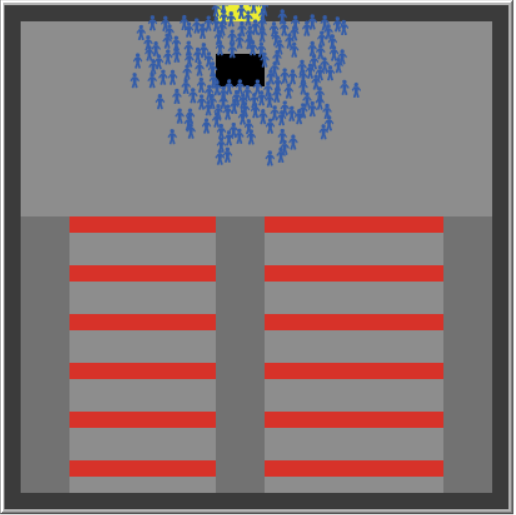
\includegraphics[scale=0.35]{obstacle.PNG}
  \centering
	\caption{Avec obstacle devant la sortie }
 	\label{pic: obstacle}
\end{figure}

La moyenne obtenue fut : 213.15 secondes
Certaines simulations ont eurent des données extrêmes ({\em 265 secondes par exemple}) car il arrivait que les turtles proches de la sortie se bloquaient mutuellement et plusieurs ticks passaient sans qu'elles ne bougent. Mais cela restait des cas rares ({\em 1 ou 2 simulations sur les 20}).

\begin{figure}[H]
	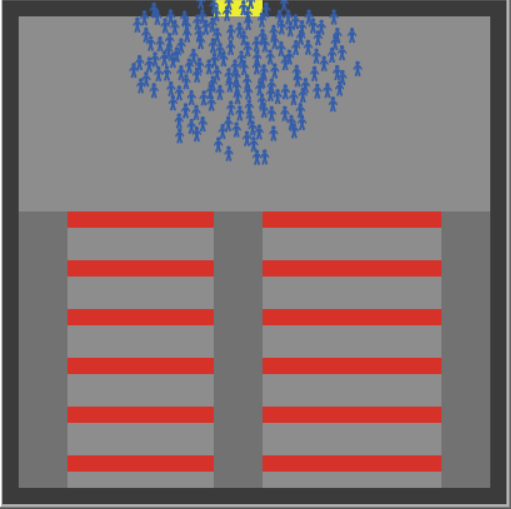
\includegraphics[scale=0.35]{sansobstacle.PNG}
  \centering
	\caption{Sans obstacle devant la sortie }
 	\label{pic: sans obstacle}
\end{figure}
La moyenne obtenue fut : 224.7 secondes.
Donnant ainsi un écart de plus de 11 secondes. Cette fois les turtles se bloquaient mais cela ne venait pas d'un bug mais du grand nombre de turtles présentes au même endroit. \\\\
Chacun de ses cas et les données obtenues nous amènent donc à l'analyse de nos résultats.

\section{Discussion} 
Dans un premier temps, certain de nos résultats étaient attendus, c'est le cas du nombre de sortie ainsi que la densité. \\

Néanmoins, il est essentiel de constater que la vitesse d'évacuation est doublée lorsque le nombre de sorties l'est aussi. Un nombre trop important de celles-ci ne changerai pas significativement la vitesse d'évacuation. Ainsi il est facile de remarquer que deux sorties est idéal d'un point de vue sécuritaire. Leur disposition, plus précisément leur emplacement apportent beaucoup à l'optimisation de l'évacuation. Il faut qu'elles soient symétriquement opposées et assez espacées l'une de l'autre afin de séparer les individus en deux groupes distincts et distants.\\

Quant à la densité, sa quasi-linéarité avec le temps d'évacuation amène à la conclusion simple qu'une salle dispose d'une capacité maximale à respecter. Dans le cas contraire la lenteur de l'évacuation due à la forte densité met alors en danger beaucoup d'individus. \\

L'enjeu le plus important de la modélisation est sûrement l'interprétation des pertes lors de l'incendie. En effet lorsque le feu démarre proche de sorties, on remarque une dispersion du nombre de morts atteignant des extrêmes maximaux ({\em 16 morts}) soit environ 13\% des individus. Néanmoins quand l'incendie démarre proche des escaliers, entre les sièges, le nombre de morts reste relativement bas entre 1 et 4 morts. On remarque facilement que le danger augmente fortement lorsque un incendie démarre près des sorties où les gens se dirigent. La solution pour éviter de fortes pertes serait donc de disposer de nombreux extincteurs ou/et détecteurs de fumée proches des sorties pour éteindre rapidement et efficacement le feu. Ce qui empêcherait de les obstruer.\\

Enfin concernant l'obstacle, on remarque son influence en cas de congestion. En effet dans la vie réelle ({\em moins explicité dans la simulation}) une forte congestion entraine des sur-accidents. L'obstacle intervient alors afin de séparer le flux important d'individus en deux, et ce juste avant la sortie. Il permet alors d'obtenir une situation convexe où les personnes ne se bloquent pas. L'évacuation devant la sortie est alors fluide évitant des chutes pouvant ralentir son passage. \\\\
Toutes ces interprétations nous permettent de répondre clairement à notre question scientifique posée. On obtient alors une modélisation optimale où le nombre de pertes humaines restes relativement faible. Néanmoins de nombreuses limites viennent apporter des contre-arguments de notre modéle..

\section{Limites}
En effet elle comporte évidemment des défauts et des limites. Que cela vienne d'hypothèses simplificatrices ou bien même du code de la simulation.

Pour commencer, on pourra notifier que notre simulation créer un effet de congestion moyen. Que ce soit à cause du faible nombre d’individus ou bien même de la façon dont la  réactions des turtles ({\em individus}) est codée. Il pourrait être nettement améliorer et donc insister d’autant plus sur l'influence des obstacles devant les sorties. 

L’hypothèse simplificatrice des individus tous identiques ({\em vitesse et taille}) et celle qui fait que personne ne peut se bousculer nous éloigne des faits réels. En effet, un enfant ne pourrait pas se frayer un chemin en poussant les autres comme le ferait un adulte et qu’un individu âgé ne pourrait atteindre la sortie aussi vite qu’un plus jeune et risquerait de se blesser gravement en tombant au sol. Tout cela n’a pas lieu dans notre simulation. 

Le réalisme du feu est absent de notre modèle : si le feu touche une turtles, aussitôt celle-ci meurt, là ou dans la vie réelle le feu ne tuerai pas instantanément et qu’un individu éteindrai les flammes qui le consument.

Enfin, un limite assez secondaire, d'autres représentations de salle seraient possible. Par exemple un autre endroit ({\em amphithéâtre, open-space}), mais également d’autres emplacement de sortie et d’autres taille de salle. 

\section*{Conclusion et perspectives} 

Comment optimiser une évacuation?
Tout au long de ce projet nous avons suivi un cheminement scientifique qui, en partant d'un problème concret, nous a mené à des solutions.
Pour les obtenir, nous avons tout d'abord analysé le problème pour en dégager les principaux aspects, puis nous l'avons modélisé pour déduire des réponses au travers de simulations.

Nous avons ainsi pu observer comment se comporterait une foule dans le cas d'une évacuation d'urgence, et comment des paramètres tels que la densité, l'emplacement du danger ainsi que le nombre de sorties et la présence d'obstacle pour séparer le flux allaient jouer sur le temps d'évacuation. Tout cela permet donc de répondre aux critères d'optimisation de l'évacuation.

Nos travaux ont donc permis de mettre en évidence les paramètres influant sur la sécurité et la survie des individus en cas de dangers et peuvent donc servir de prototype dans le domaine sécuritaire.

Évidemment, nos travaux restent tout de même peu précis et peu avancés du à la limite de temps dont nous disposions et de la faible maitrise du logiciel {\it Netlogo}. Elle reste néanmoins une preuve de l'importance d'organiser d'une salle pouvant contenir plus d'une centaine de personnes, afin de garantir la survie de ceux-ci.

\bibliographystyle{named}
\bibliography{ijcai13}
\end{document}